\documentclass{acm_proc_article-sp}
\usepackage{graphicx}
\usepackage{float}
\usepackage{epstopdf}
\usepackage{hyperref}
\usepackage{flushend}

\begin{document}

\title{A Comparison of Scheduling Algorithms}
\numberofauthors{1}
\author{
\alignauthor
Samuel Jackson\\
       \affaddr{Aberystwyth University}\\
       \email{slj11@aber.ac.uk}
}
\date{\today}

\maketitle

\begin{abstract}
This paper analyses four different scheduling algorithms (namely Shortest Remaining Time, First Come, First Served, Round Robin and Lottery Scheduling) to compare and contrast their performance in a simulated environment and evaluate their strengths and weaknesses. This was done by creating a set of experimental test files containing jobs exhibiting a variety of features likely to be present in a real world scheduling environment and running these on the simulator. The results showed a clear trend towards time slice based schedulers having a higher mean job duration but a lower idle time. The reverse appeared to be exhibited by queue based approaches. By analysing the results of these tests it was possible to determine the major differences between the four approaches, where a clear trade off between throughput, mean job duration, and context switches versus idle time and the possibility of starvation occurred.

\end{abstract}

% A category with the (minimum) three required fields
\category{D.4}{Operating Systems}{Process Management}[Scheduling]
%A category including the fourth, optional field follows...
\category{D.2.8}{Software Engineering}{Metrics}[complexity measures, performance measures]

\terms{Algorithms, Performance, Measurement}

\keywords{Algorithms, Scheduling, Performance, Lottery Scheduling, Shortest Remaining Time, Round Robin}

\section{Introduction}
This report aims to examine the differences between four approaches to scheduling algorithms that are widely used in systems throughout computer science where multiple tasks require computation in parallel. Scheduling algorithms are used to organise and prioritise jobs of computation according to a set scheme which deals with the issues such as throughput, job turnaround and context switching.

The scheduling algorithms examined here are First Come, First Served (FCFS)\cite{donaldson:scheduling}\cite{ozdogan:scheduling}, Shortest Remaining Time (SRT)\cite{donaldson:scheduling}\cite{ozdogan:scheduling}, Round Robin\cite{donaldson:scheduling}\cite{ozdogan:scheduling} and Lottery scheduling\cite{petrou:lottery} which were chosen because they all exhibit characteristics which make them suitable for different situations. The former three are deterministic in nature while lottery scheduling is non deterministic. FCFS will work on the first job given to the scheduler until it finishes or is blocked for I/O. In which case it will be returned to the back of the queue. SRT takes a simple priority queue based approach where jobs are ordered according to the amount of time left before they finish processing. Round Robin uses equal time slices to share processing time between every job in the queue. Finally, Lottery scheduling uses probabilistic methods to give higher priority jobs a greater likelihood of being selected. In the implementation used in this report Lottery scheduling treats lower priorities as being of greater importance.

\section{Methodology} 
\label{methodology}
To thoroughly test the performance of the algorithms, each of the schedulers were exercised using a set of data files each specifically designed to test different properties important to scheduling algorithms. This includes files which contain a heavy amount of I/O processing, zero I/O processing, a test where all job priorities are the same, and some general test data. Test data that is heavy in I/O processes exercises how well an algorithm handles a high level of context switching due to jobs being blocked for reading or writing. The data file with a low level of I/O is used to evaluate the performance of the scheduler in situations which would not require I/O. A file where all priorities are the same is used to help evaluate lottery scheduling (which schedules according to priority) to evaluate its worst case performance.

Th method used to test each algorithm was to run it with each of the supplied generic and custom data files to evaluate how each algorithm handles specific aspects of scheduling. The results are then compared against one another using six attributes important to scheduling algorithms (mean duration, total CPU time, number of context switches, idle time and the duration of the first job to finish and time for first job to finish) in order to show how each algorithm performed both with generic test data and specific test data to gauge an idea of where each scheduler excels and where it does not.

Because lottery scheduling is non-deterministic it required a slightly different approach to testing that involved an extra step. Lottery scheduling gives different results on each run. Therefore in order to evaluate an average run an automated simulator (code included with alongside the schedulers) was created to simulate 10,000 runs of the algorithm per test file. The results of this data could then be averaged out to representatively compare lottery scheduling's general case performance with the performance of the other algorithms. It is this average which has been used in comparisons with the other schedulers in the following section and it is therefore important to remember that the value generated by lottery scheduling will vary, but will on average behave like the value given.

\section{Results}
\label{results}
This section details the outcomes of testing each of the algorithms using the data files outlined in section \ref{methodology} to measure five key attributes important to scheduling algorithms. As mentioned in the preceding section, the values used with lottery scheduling are the mean results of 10,000 tests.

\subsection{Mean Duration}
\label{results-duration}
Mean duration is the average amount of time that a scheduled job takes to finish processing. Figure \ref{fig:duration} shows that the mean duration time across all tests and algorithms was fairly consistent, with Shortest Remaining Time (SRT) having the lowest mean duration in all tests. Round Robin scheduling showed the worst performance of the four with mean durations slightly above those of FCFS and Lottery scheduling, both of whom presented mixed results depending on the test. The mean duration appears to spike on test 3 and on the test with no I/O blocking, although SRT appeared to show a significantly lower mean duration time for the no I/O test than the other schedulers.


\begin{figure}[H]
\centering
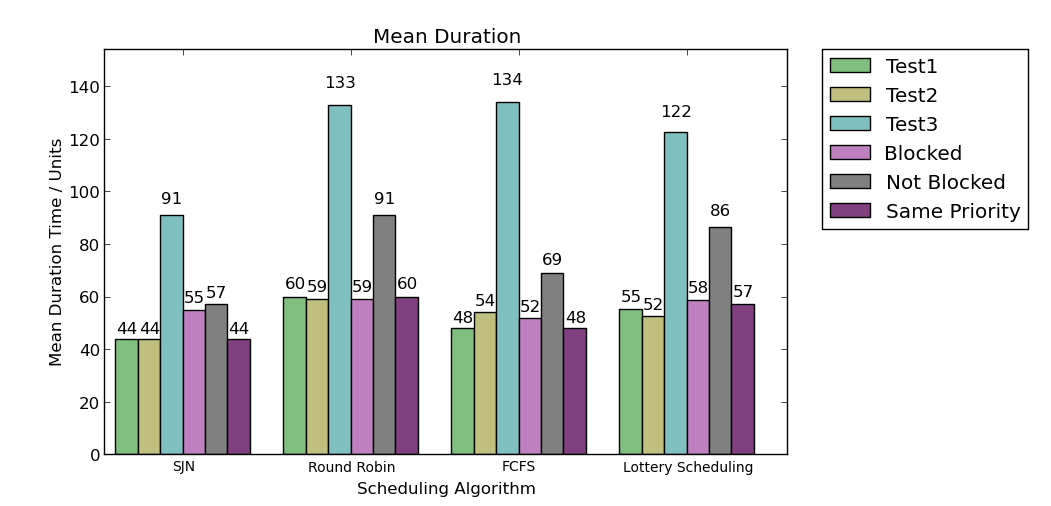
\includegraphics[width=0.5\textwidth]{duration.png}
\caption{Mean Job Duration across all tests and algorithms}
\label{fig:duration}
\end{figure}

\subsection{CPU Time}
CPU time is the number of CPU ticks that each algorithm performs in total in order to complete all of the jobs. Figure \ref{fig:cpu-time} shows that the CPU times were also fairly consistent across all tests with Round Robin besting or equalling the other algorithms. Conversely, SRT performed slightly worse in this criteria than the others. Also, FCFS exhibited a higher CPU time at 191 ticks as opposed to a consistent 182 ticks for every other algorithm. 

\begin{figure}[H]
\centering
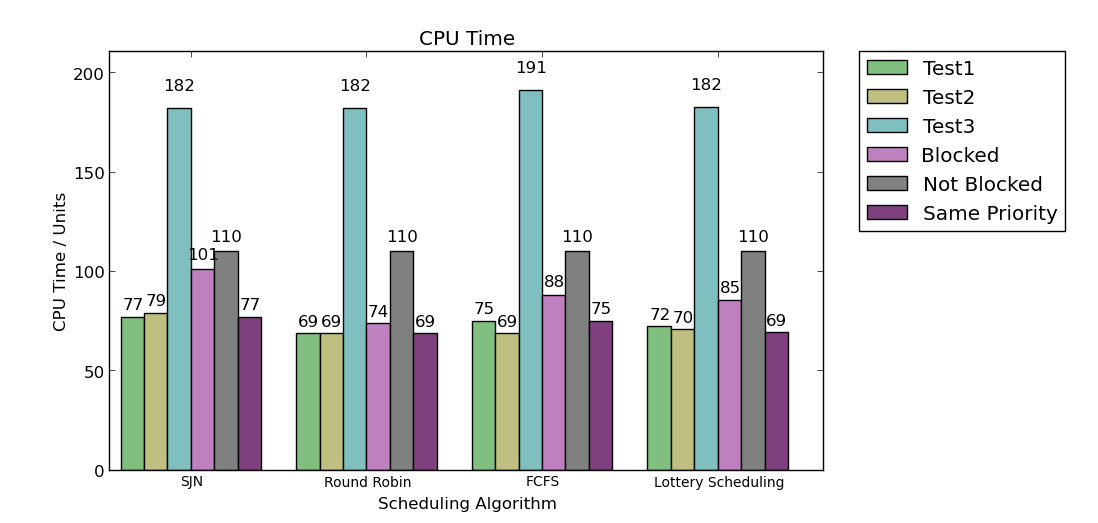
\includegraphics[width=0.5\textwidth]{cpu_time.png}
\caption{CPU time to complete processing jobs across all tests and algorithms.}
\label{fig:cpu-time}
\end{figure}

\subsection{Context Switches}
Context switches measure the number of times the algorithm manually switches between different jobs. Figure \ref{fig:ctex-switches} shows a mixed result between FCFS and SRT in terms of the number context switches made with FCFS having the lowest result on tests 1,2, the high I/O blocking test and the test with all priorities the same and SRT scoring lower on the other two tests. Round Robin had the worse performance overall with Lottery scheduling following closely behind. 

Interestingly, FCFS had a very high number of context switches on tests 3 and the non I/O blocking test when compared with its closest counterpart SRT. In fact, the SRT algorithm exhibited the lowest number of context switches in the non I/O blocking test.

\begin{figure}[H]
\centering
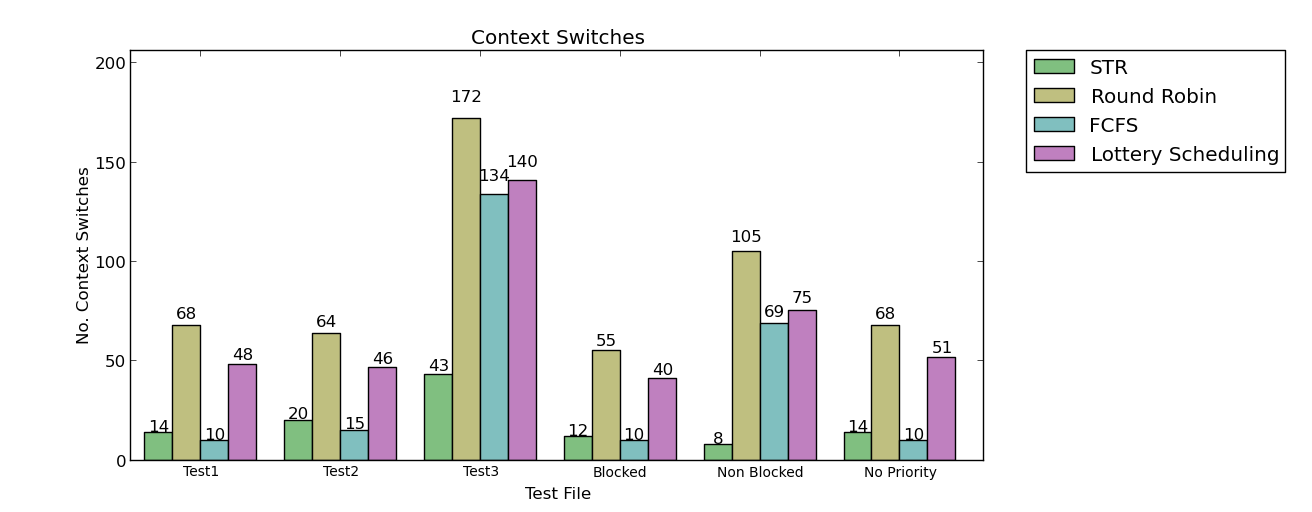
\includegraphics[width=0.5\textwidth]{ctex_switches.png}
\caption{Total number of context switches across all tests and algorithms.}
\label{fig:ctex-switches}
\end{figure}

\subsection{Idle Time}
Idle time is the number of CPU ticks that occur where there were no jobs pending within the scheduler as they were all either finished or blocked for I/O. Figure \ref{fig:idle-time} shows the total idle times for all tests as a percentage of the total CPU time which clearly shows Round Robin to be the winner with only 5\% of its time spent idle during the high I/O blocking test and 0\% idle time for every other test. Lottery scheduling performed reasonably well, while SRT and FCFS showed mixed results. Interestingly, SRT had no idle time in test 3 while FCFS had no idle time in test 2. SRT had a significantly higher idle time during the non blocking I/O test with 31.7\% of its CPU time spent idle. The high I/O blocking test proved to show the largest impact on the idle time compared with the other tests.

\begin{figure}[H]
\centering
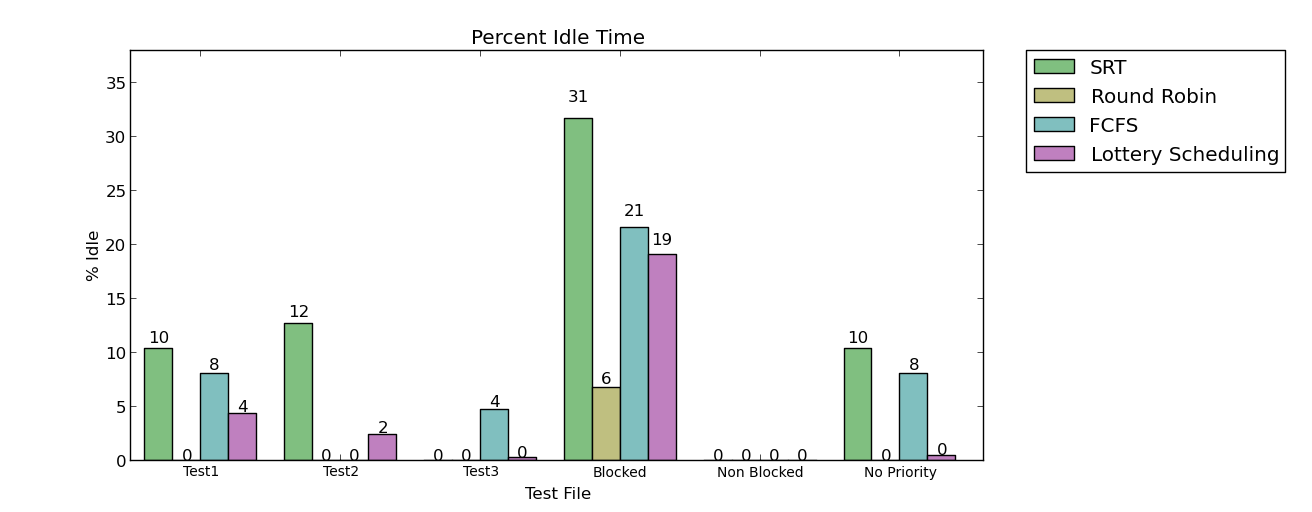
\includegraphics[width=0.5\textwidth]{idle_time_per.png}
\caption{Total idle time as a percentage of CPU time across all tests and algorithms.}
\label{fig:idle-time}
\end{figure}

\subsection{First Job Finish Time}
\label{results-fstjob-time}
First job finish time is the total number of CPU cycles from the start of scheduler execution for the first job to finish processing. Figure \ref{fig:fstjob-time} shows the time for the first job to finish across all tests and algorithms. From this it can be seen that STR and FCFS were generally the best performers in this category with STR taking a consistent 15 cycles across every test. Round Robin showed the worst performance in very test with lottery scheduling following closely behind.

\begin{figure}[H]
\centering
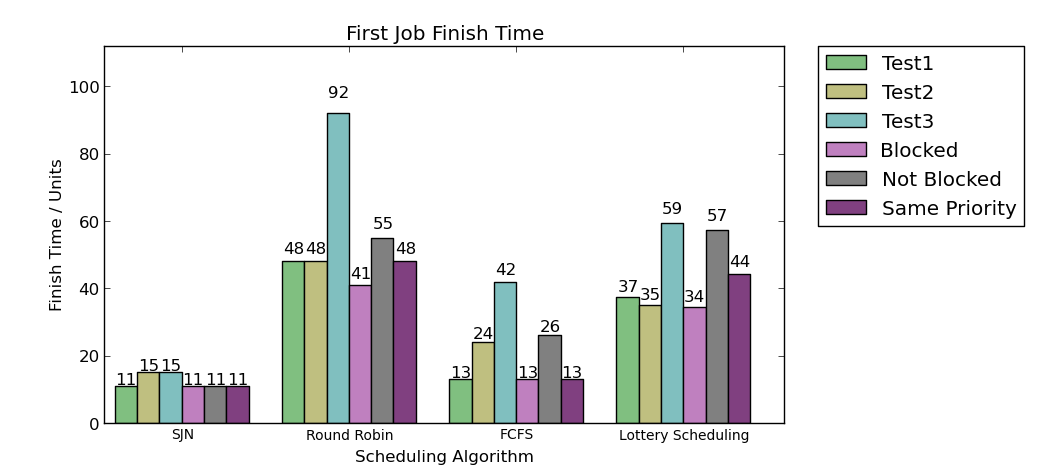
\includegraphics[width=0.5\textwidth]{fstjob_time.png}
\caption{Time for the first job to finish across all tests and algorithms.}
\label{fig:fstjob-time}
\end{figure}

\subsection{First Job Duration}
\label{results-fstjob-duration}
This final section shows the duration that the first job spends in the scheduler across all tests. Figure \ref{fig:fstjob-duration} clearly shows that SRT to be significantly faster than both Round Robin and Lottery scheduling as well as being generally faster than FCFS. Round Robin has the slowest performance in this category, with test 3 taking 92 cycles in order to finish the first job compared to just 15 cycles using SRT.
\\\\\\
\begin{figure}[H]
\centering
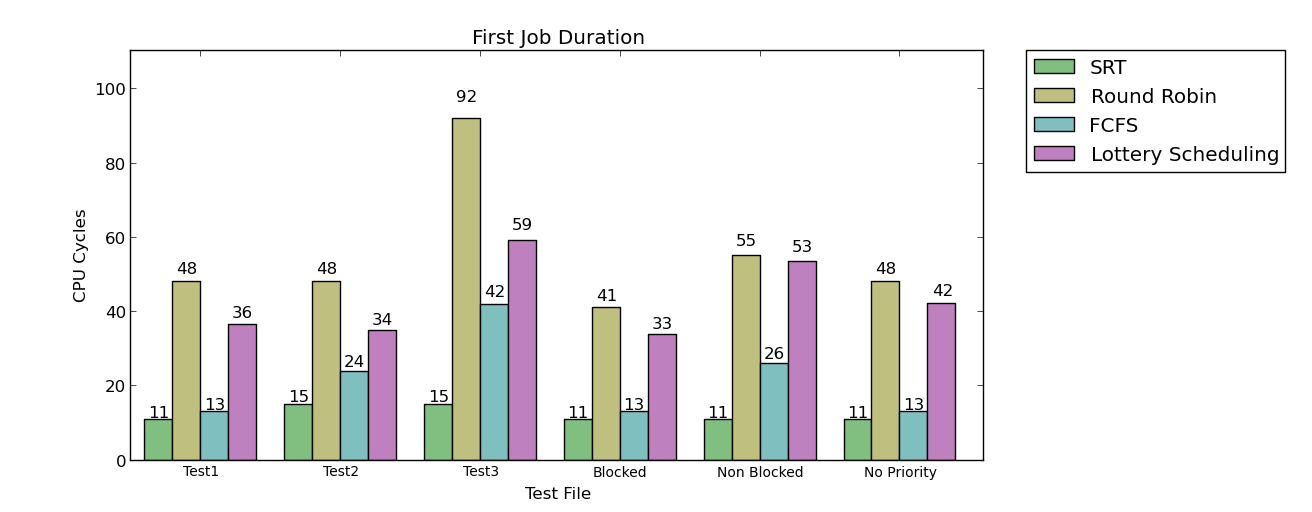
\includegraphics[width=0.5\textwidth]{fstjob_duration.png}
\caption{Time for the first job to finish across all tests and algorithms.}
\label{fig:fstjob-duration}
\end{figure}

\section{Discussion}
This section discusses the results presented in section \ref{results} to examine the strengths and weaknesses of each algorithm in each of the following categories: first job finish time, mean job finish time, and overall processing time.

\subsection{First Job Finish Time}
The results shown in subsections \ref{results-fstjob-time} and \ref{results-fstjob-duration} generally suggest that the Shortest Remaining Time algorithm is the fastest at finishing the first job. This seems logical because SRT prioritises new and returning jobs by the amount of processing that they have left and therefore the SRT will put the shortest jobs towards the start of the queue and longer jobs towards the back. This means that regardless of the test data, SRT puts the shortest job at the front and this job will get immediate processing and (providing it does not require an I/O block, will finish in the shortest possible amount of time.

This is in contrast with the other three algorithms which do not order their jobs according to time remaining. Round Robin scheduling had the worst results in this category. Again, this seems logical because Robin Robin allocates equal CPU time slices to each job regardless of its size or priority, suggesting that the shortest job will take much longer to finish as processing time must be shared equally between this job and the other jobs in the queue. This is confirmed by the data shown in figure \ref{fig:fstjob-time} where the first job in test 3 (by far the longest set of jobs) takes much more time to finish than in any other test. The slightly higher result for the test with no I/O blocking shows a higher finishing time for the first job. This is presumably because the less jobs that get blocked means there are more jobs in the queue and the longer a job must wait for more CPU time.

The First Come, First Served algorithm appeared to be the second best choice after SRT with it competing with FCFS in first job finish time and coming close on three tests in first job duration. However, as with Round Robin, FCFS does not prioritise the shortest job, but rather accepts the first job added to the queue and and continues working on it until it finishes or, if it becomes blocked for I/O, it is returned to the back of the queue. Therefore the time taken for the first job to finish in FCFS depends upon two factors which are the size of first job in the queue and whether the job will become blocked for I/O. 

It is for these reasons that FCFS is sometimes faster in some tests in subsection \ref{results-fstjob-time} but STR is always faster in the tests in subsection \ref{results-fstjob-duration}. FCFS is occasionally faster because STR will swap to another job if the current one becomes blocked but (unlike FCFS) will swap back to the shortest job after it has become unblocked. FCFS on the other hand will place the returning job (which may be shorter) to the back of the queue. If the first and second jobs added to a FCFS scheduler are quite small and the first becomes blocked FCFS will process the second until finished while STR would swap back to the first after it become unblocked.

If the job becomes blocked for I/O then it will be added to the back of the queue and will have to wait for all of the processes in front of it to finish before it will get CPU time again. If there are lots of jobs that require being blocked for I/O for short periods of time (such as in test 3) then FCFS will begin to cycle through jobs rather than concentrating on a single job until it's done.

Lottery scheduling appeared to come off as the average case in the results presented in subsection \ref{results-fstjob-time}. The implementation of lottery scheduling used here does not prioritise jobs according to their length (although it could be implemented to prioritise by job length) but instead uses the priority assigned to be job inside the testing file (which is presumably a arbitrary number according to the current importance of the job on the system). Because jobs are weighted according to priority and not the size of the job, and because this implementation is pre-emptive, there is no guarantee about the length of time taken for the first job to finish. The speed that the initial job will finish in is decided by a jobs priority and random chance. Because this implementation is random and pre-emptive, Lottery scheduling made many frequent switches between jobs and therefore had a higher first job finish time but because some jobs were weighted more highly than others would still perform better than Round Robin.

\subsection{Mean Job Duration Time}
When considering the mean time to finish a job, It appears that the Shortest Remaining Time algorithm proves to be the best option. Referring to figure \ref{fig:duration} we can see that on average SRT had the shortest mean time to finish a job compared with any other algorithm. This would appear to coincide with expectations as the SRT algorithm always attempts to bring the shortest job to the front of the queue which means they finish very quickly thus pulling the mean duration down. However, this comes with the caveat that longer processes can be starved of CPU time when there are lots of small jobs. This could be a particularly nasty problem if there is a constant stream of small jobs being added to the queue as this would force the mean duration to grow much higher as longer jobs would have to wait a long time for CPU time.

The second best performing algorithm in this section was First Come, First Served which exhibited only a slightly higher mean durations across all tests except in the case of test 3 where is was the worst performer and test 2 where it was narrowly beaten by lottery scheduling. Once again this seems to correlate with predictions. FCFS processes jobs as they arrive, so a queue with only a few short jobs will perform fairly similarly to SRT. However, when there are a lot of jobs on the queue the algorithms performance begins to deteriorate as longer processes begin to hold the CPU meaning shorter or higher priority jobs get starved of resources. Also, because of the lack of prioritisation, jobs that have been blocked are returned to be back of the queue regardless of the amount of processing left which means nearly complete tasks can be placed right at the back of the queue thereby increasing their duration.

As for the other two tests, figure \ref{fig:duration} shows that Lottery scheduling came a narrow third with Round Robin coming in last. The reason for this is most likely because these two algorithms are more orientated around sharing CPU resources according to time or priority rather than attempting to gain maximum throughput like SRT, making it a more appropriate choice when maximum throughput is not essential.

The data shown in \ref{fig:duration} shows that the difference in mean duration increases between the shorter tests (1 \& 2) and the longer test 3. Looking at the results shown in figure \ref{fig:fstjob-time} we can see that Round Robin had the highest first job finish time. These two points show that the mean duration is affected in Round Robin scheduling because the mean is altered due to jobs generally taking a longer time to finish than with the other scheduling algorithms. It is suggested that because jobs are cycled through in the order they are added, the shorter jobs are not finished as quickly as with other approaches as they are constantly waiting for time on the CPU and hence upping their duration and therefore the mean duration.

Finally, Lottery scheduling shares similar issues with Round Robin in the test of mean duration. Lottery scheduling has a higher mean duration than SRT and FCFS because its approach to scheduling uses randomness and the priority of the job (which has nothing to do with job size) to select which job should get processing time next. This means that, like Round Robin, shorter jobs may not be prioritised CPU time and therefore will generally take longer than with SRT. However, unlike Round Robin, CPU is not shared equally among all jobs but is weighted towards more important ones. This coupled with the element of randomness ensuring that all jobs are potentially allotted processing time makes the likely mean duration of Lottery scheduling difficult to quantify, but generally appears to be slightly quicker than with Round Robin in the average case, but because of Lottery scheduling being non-deterministic the performance may vary per run.

\subsection{Overall Processing Time}
When comparing the overall processing time taken to complete the tests as seen in figure \ref{fig:cpu-time}, Round Robin appears to be marginally better than the other algorithms where it either equals or surpasses every other scheduler in CPU time. If we compare this evidence with the data shown in figure \ref{fig:idle-time} it can be seen that Round Robin wastes a very small amount of time being idle compared with the other three algorithms. This suggests that while jobs scheduled using Round Robin take (on average) longer to complete, Round Robin is much more efficient in the use of this time. This coincides with expectations because Round Robin does not waste time with jobs that have been blocked for I/O but will continue cycling through any other available jobs.

Lottery scheduling was the second best performer for overall with most values CPU usage times falling between those of Round Robin and FCFS. The explanation for this can again be seen by turning to \ref{fig:idle-time} where it can be seen that lottery scheduling had the second lowest idle time of any scheduler, suggesting that there is positive correlation between the amount of total overall processing time for a scheduler and the amount of time it spends idle.

In contrast, the worst performing scheduler in this category was Shortest Remaining Time which had the highest total CPU time in every test except test 3. Comparing this with the results of the idle testing we can see that the correlation between processing time and idle time holds once again. In particular, on the high number of blocking jobs test SRT spent a massive 31.7\% of its total execution time being idle; causing a massive waste of system resources.

According to the data in figure \ref{fig:cpu-time} all of the scheduling algorithms performed exactly the same on the test with no I/O blocking which strongly agrees with the prior argument that the major factor affecting the overall processing for a set of jobs is what a scheduling algorithm does when a job is blocked for I/O and how much of its time is spent idle.

Interestingly, there also appears to be a negative correlation between the number of context switches a scheduler makes and its overall processing time. Figure \ref{fig:ctex-switches} shows that Round Robin had the most context switches in every category while SRT consistently had the lowest number of context switches. Both Lottery scheduling and FCFS also appear to fit with this trend. However, it appears that the number of context switches made is mostly lower for all scheduling algorithms on the test with a high amount of I/O blocking. This could be explained by the fact that the high I/O blocking test blocks jobs for a long period of time rather than making many short blocks meaning that the schedulers are able to make a single context switch and forget about the job until it returns. By contrast test 3 showed a high number of context switches due to having many jobs that required being blocked for a small portion of time.

Therefore, in summary of this section, it appears for the collected data that there is a positive correlation between the overall processing time of a set of jobs and the the idle time as well as a negative correlation between the overall processing time and the number of context switches a scheduler makes. It is suggested that making more context switches reduces the amount of time that a scheduler spends being idle and hence the faster it finishes processing. However it is worth noting that the data collected from the simulated runs in no way accounts for any overheads that might occur when performing a context switch which could be considerable depending on the system and implementation.

\section{Conclusions}
To summarise what has been illustrated by the data analysed in the preceding sections of this document, it can be seen that there are many key factors affecting scheduling algorithm performance. The way that a scheduler manages these factors defines the type of scheduling problem it can be used to solve but the correct solution to any problem will always remain implementation specific.

Shortest Remaining Time appears to be best suited to applications that require short processes to be handled as quickly as possible to allow for a high level of throughput and a minimisation on the average job waiting time. SRT generally has a very low number of context switches compared with the other algorithms listed here meaning that in real world applications the overheads associated with a context switch would be kept to a premium. However, these benefits come at the cost of a higher amount of idle time and therefore a higher overall processing time is more likely. The fact that shorter jobs will also be brought closer to the front of the queue means that under a heavy load longer process are likely to become starved of processing time.

First Come, First served also appears to be suited to situations that require a very low number of context switches and works well when jobs are mostly short. FCFS runs into issues when longer jobs which do not get blocked for I/O are present in the queue as they they begin to hold the CPU's time. However it does have the advantage of SRT accounting for starvation providing all jobs will eventually complete (although the waiting time may be very high) as every job will get to execute. There may however, be the illusion of starvation if a very long job (such as a process that is constantly left running for days) is added to a FCFS scheduler.

Round Robin scheduling has a slower mean job duration as jobs spend longer waiting in the queue but in these tests proved to be slightly faster than the other algorithms due the the low amount of time spent idle. Unlike SRT, Round Robin solves the problem of starvation because every process is given an equal amount of execution time meaning that both long and short jobs receive processing time, even in a system under heavy load. However, the largest problem with Round Robin is the high context switching overhead as jobs get switched after every CPU cycle.

An interesting area for further investigation with Round Robin scheduling would be to up the amount of CPU cycles a job gets before it is swapped to the back of the queue (currently a job only gets one cycle). This would produce a drop in the number of context switches the scheduler has to make thereby reducing the overhead. However, by allowing multiple CPU cycles it could cause scheduler to begin to perform more like FCFS because (if the time slice is high enough) the whole job could finish before being swapped out meaning that the first job in the queue will generally be the first to finish. Therefore the key to  the optimum performance of a Round Robin algorithm is likely to be finding the "sweet spot" that minimising the number of context switches while still providing jobs with fair access to processing time.

Lottery scheduling is the only scheduling approach of the three that uses the priority supplied with each test file to select which job should be processed next. The implementation used here is weighted meaning that more important jobs are more likely to be selected. This implementation is also pre-emptive, meaning that a lottery is run every time a job is added and also when a job is returned meaning that it behaves (as shown in the test data) generally like Round Robin. The weighting means that less context switches are made and therefore jobs appear to get a higher slice of CPU time in proportion to there weighting.

However, lottery scheduling can be made to work like other scheduling algorithms depending on how it is tuned. For example, it could easily be made to work in a similar fashion to Shortest Remaining Time if the weights of the jobs were based on the amount of time left before the job completes but would still not be exactly the same because there is a chance that jobs with a longer time could jump to the front. Therefore while the exact throughput speed offered with SRT could never be achieved, Lottery scheduling can be made to approximate closely to SRT but with the added benefit of solving the issue of starvation as there is always a chance jobs with higher time remaining to taking over. This will of course mean that it would also still have a higher context switching overhead than SRT.

The performance of Lottery scheduling can vary between runs. This means that while it can be made to approximate other algorithms the outcome of scheduling can be highly variable. In the data presented in section \ref{results} the average result was presented, but the actual value can vary depending on the the random value generated. Therefore while the algorithm will generally run within a couple of cycles of the mean value it can be much worse or much better. This means that Lottery scheduling may not be the best approach to take when consistent performance is key to scheduling success. It is also worth noting that the implementation used here relies on the Java's own pseudo-random number generator and so may not produce truly random results over time. However for simple purposes a pseudo-random generator should give sufficiently random results.

\section{Executive Summary}
In summary of this document, it can be seen that there are a variety of different approaches that can be taken to the problem of scheduling. Each of the algorithms in this document aim to handle factors affecting the performance of scheduling in different ways. 

Round Robin cycles through the jobs to give each job a slice of time on the CPU. In doing this Round Robin minimise the amount of time that it spends being idle, but at the cost of a slightly higher mean job duration and a higher number of context switches.

Similarly the Lottery scheduling implementation performed in a way that was similar to Round Robin, but because of weights allocated to higher priority jobs had a lower number of context switches and was generally slightly faster than Round Robin. 

In contrast Shortest Time Remaining showed a high throughput and hence a slightly lower mean duration but its overall processing time proved to not be significantly better than the other schedulers due to long periods spent being idle. SRT also exhibited a much lower number of context switches and hence would have a lower computational overhead in a real world application.

First Come, First Served generally performed like Shortest Time Remaining but generally had a slower mean duration as longer processes tended to hold the CPU because of the lack of job prioritisation. The lack of prioritisation caused it to have idle times that were similar in scale to SRT as well as a smaller number of context switches.

In conclusion this document has shown that there is a trade off between the average job duration and the number of context switches made against the amount of time spent being idle and the possibility of process starvation. The choice of scheduler relies heavily on the amount to which these factors affect the larger system as a whole.

\section{Acknowledgements}
The author wishes to thank Richard Shipman (rcs@aber.ac.uk) for providing the supporting simulation code and GUI.


\balancecolumns
\bibliographystyle{abbrv}
 % sigproc.bib is the name of the Bibliography 
\bibliography{sigproc}

\end{document}